\documentclass[11pt]{standalone}
\usepackage[usenames]{color} %used for font color
\usepackage{amssymb} %maths
\usepackage{amsmath} %maths

\usepackage[no-math]{fontspec}
\usepackage{unicode-math}
\setmainfont{Lato}
\setmathfont{Stix Two Math}

\usepackage{pgf,xcolor}
\definecolor{itwm_blue_04}{HTML}{005A94}
\definecolor{itwm_red}{HTML}{C00000}
\definecolor{itwm_yellow}{HTML}{FFEC7F}

\usepackage{tikz}
\usetikzlibrary{shapes.misc, shadows, decorations, arrows}
\usetikzlibrary{backgrounds}
\usetikzlibrary{calc}
\usepackage{pgfplots}
\pgfplotsset{compat=newest}
\usepgfplotslibrary{fillbetween}
\usepackage{tikzpagenodes}

\begin{document}
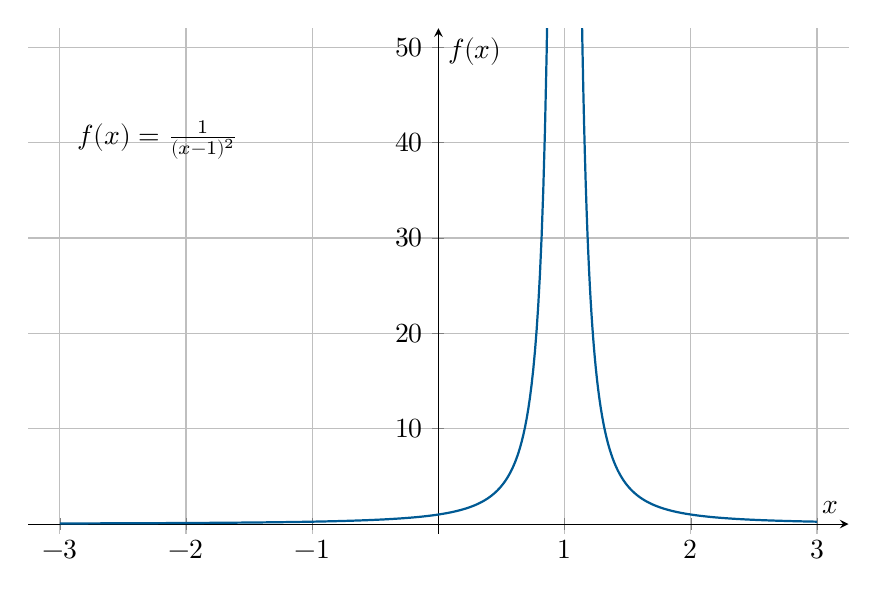
\begin{tikzpicture}
\begin{axis}[
    domain=-3:3,
    axis lines = center,
    xlabel = {$x$},
    ylabel = {$f(x)$},
    height=8cm, width=12cm, 
    xmin=-3.25, xmax=3.25, ymin=-1, ymax=52, 
    xtick={-3, -2,...,3},
    ytick={0, 10,...,50},
    grid = both
]
\addplot[draw=itwm_blue_04, samples=300, thick, name path=f, domain=-3:0.95]{1/(x-1)^2};
\addplot[draw=itwm_blue_04, samples=300, thick, name path=f, domain=1.05:3]{1/(x-1)^2};
\end{axis}
\node [anchor=west] (note) at (0.5,5) {$f(x)=\frac{1}{(x-1)^2}$};
\end{tikzpicture}
\end{document}